\documentclass[journal]{IEEEtran}
\usepackage[a5paper, margin=10mm, onecolumn]{geometry}
\usepackage{lmodern}
\usepackage{tfrupee}
\setlength{\headheight}{1cm}
\setlength{\headsep}{0mm}

\usepackage{gvv-book}
\usepackage{gvv}
\usepackage{cite}
\usepackage{amsmath,amssymb,amsfonts,amsthm}
\usepackage{algorithmic}
\usepackage{graphicx}
\usepackage{textcomp}
\usepackage{xcolor}
\usepackage{txfonts}
\usepackage{listings}
\usepackage{enumitem}
\usepackage{mathtools}
\usepackage{gensymb}
\usepackage{comment}
\usepackage[breaklinks=true]{hyperref}
\usepackage{tkz-euclide}
\usepackage{listings}
\def\inputGnumericTable{}
\usepackage[latin1]{inputenc}
\usepackage{color}
\usepackage{array}
\usepackage{longtable}
\usepackage{calc}
\usepackage{multirow}
\usepackage{hhline}
\usepackage{ifthen}
\usepackage{lscape}
\usepackage{xparse}


\bibliographystyle{IEEEtran}

\title{2.8.25}
\author{EE25BTECH11043 - Nishid Khandagre} % Replace with your name

\begin{document}
\maketitle

\renewcommand{\thefigure}{\theenumi}
\renewcommand{\thetable}{\theenumi}

\numberwithin{equation}{enumi}
\numberwithin{figure}{enumi}

\textbf{Question}:\
If $\vec{A}$, $\vec{B}$, $\vec{C}$ are mutually perpendicular vectors of equal magnitudes, show that $\vec{A} + \vec{B} + \vec{C}$ is equally inclined to $\vec{A}$, $\vec{B}$ and $\vec{C}$.

\textbf{Solution: }
Given:
    \begin{align}
    \vec{A}^\top \vec{B} &= 0 \\
    \vec{B}^\top \vec{C} &= 0 \\
    \vec{C}^\top \vec{A} &= 0
    \end{align}
    
    \begin{align}
    \norm{\vec{A}} = \norm{\vec{B}} = \norm{\vec{C}} = k
    \end{align}
    This implies:
    \begin{align}
    \vec{A}^\top \vec{A} &= \norm{\vec{A}}^2 = k^2 \\
    \vec{B}^\top \vec{B} &= \norm{\vec{B}}^2 = k^2 \\
    \vec{C}^\top \vec{C} &= \norm{\vec{C}}^2 = k^2
    \end{align}

Let 
\begin{align}
\vec{R} = \myvec{\vec{A} + \vec{B} + \vec{C}}
\end{align}

The cosine of the angle $\theta$ between two vectors $\vec{X}$ and $\vec{Y}$ is given by 
\begin{align}
\cos \theta = \frac{\vec{X}^\top \vec{Y}}{\norm{\vec{X}}\norm{\vec{Y}}}
\label{eq:equation}
\end{align}

\begin{align}
\norm{\vec{R}}^2 &= \vec{R}^\top \vec{R} \\
&= \myvec{\vec{A} + \vec{B} + \vec{C}}^\top \myvec{\vec{A} + \vec{B} + \vec{C}} \\
&= \myvec{\vec{A}^\top + \vec{B}^\top + \vec{C}^\top} \myvec{\vec{A} + \vec{B} + \vec{C}} \\
&= \vec{A}^\top \vec{A} + \vec{A}^\top \vec{B} + \vec{A}^\top \vec{C} + \vec{B}^\top \vec{A} + \vec{B}^\top \vec{B} + \vec{B}^\top \vec{C} + \vec{C}^\top \vec{A} + \vec{C}^\top \vec{B} + \vec{C}^\top \vec{C} \\
&= \norm{\vec{A}}^2 + 0 + 0 + 0 + \norm{\vec{B}}^2 + 0 + 0 + 0 + \norm{\vec{C}}^2 \\
&= k^2 + k^2 + k^2 \\
&= 3k^2
\end{align}
Therefore, $\norm{\vec{R}} = \sqrt{3}k$.

Now, let $\alpha$ be the angle between $\vec{R}$ and $\vec{A}$. using \eqref{eq:equation}
\begin{align}
\cos \alpha &= \frac{\vec{R}^\top \vec{A}}{\norm{\vec{R}} \norm{\vec{A}}} \\
&= \frac{\myvec{\vec{A} + \vec{B} + \vec{C}}^\top \vec{A}}{\norm{\vec{R}} \norm{\vec{A}}} \\
&= \frac{\vec{A}^\top \vec{A} + \vec{B}^\top \vec{A} + \vec{C}^\top \vec{A}}{\norm{\vec{R}} \norm{\vec{A}}} \\
&= \frac{\norm{\vec{A}}^2 + 0 + 0}{\norm{\vec{R}} \norm{\vec{A}}} \\
&= \frac{k^2}{(\sqrt{3}k)(k)} \\
&= \frac{k^2}{\sqrt{3}k^2} \\
&= \frac{1}{\sqrt{3}}
\end{align}

Let $\beta$ be the angle between $\vec{R}$ and $\vec{B}$.  using \eqref{eq:equation}
\begin{align}
\cos \beta &= \frac{\vec{R}^\top \vec{B}}{\norm{\vec{R}} \norm{\vec{B}}}  \\
&= \frac{\myvec{\vec{A} + \vec{B} + \vec{C}}^\top \vec{B}}{\norm{\vec{R}} \norm{\vec{B}}} \\
&= \frac{\vec{A}^\top \vec{B} + \vec{B}^\top \vec{B} + \vec{C}^\top \vec{B}}{\norm{\vec{R}} \norm{\vec{B}}} \\
&= \frac{0 + \norm{\vec{B}}^2 + 0}{\norm{\vec{R}} \norm{\vec{B}}} \\
&= \frac{k^2}{(\sqrt{3}k)(k)} \\
&= \frac{k^2}{\sqrt{3}k^2} \\
&= \frac{1}{\sqrt{3}}
\end{align}

Let $\gamma$ be the angle between $\vec{R}$ and $\vec{C}$. using \eqref{eq:equation}
\begin{align}
\cos \gamma &= \frac{\vec{R}^\top \vec{C}}{\norm{\vec{R}} \norm{\vec{C}}} \\
&= \frac{\myvec{\vec{A} + \vec{B} + \vec{C}}^\top \vec{C}}{\norm{\vec{R}} \norm{\vec{C}}} \\
&= \frac{\vec{A}^\top \vec{C} + \vec{B}^\top \vec{C} + \vec{C}^\top \vec{C}}{\norm{\vec{R}} \norm{\vec{C}}} \\
&= \frac{0 + 0 + \norm{\vec{C}}^2}{\norm{\vec{R}} \norm{\vec{C}}} \\
&= \frac{k^2}{(\sqrt{3}k)(k)} \\
&= \frac{k^2}{\sqrt{3}k^2} \\
&= \frac{1}{\sqrt{3}}
\end{align}

Since $\cos \alpha = \cos \beta = \cos \gamma = \frac{1}{\sqrt{3}}$, it implies $\alpha = \beta = \gamma$.\\

Thus, $\vec{A} + \vec{B} + \vec{C}$ is equally inclined to $\vec{A}$, $\vec{B}$ and $\vec{C}$.


\begin{figure}[H]
\centering
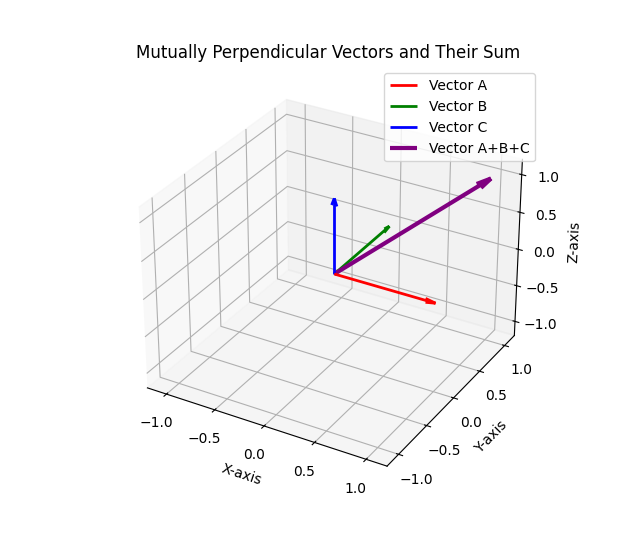
\includegraphics[width=0.8\columnwidth]{figs/fig1.png}
\caption{}
\label{fig:1}
\end{figure}

\end{document}
